\documentclass{article}
\usepackage[utf8]{inputenc}
\usepackage[left=1in, right=1in, top=1in, bottom=1in]{geometry}
\usepackage{titlesec, titling, graphicx, color, natbib, float, url}
\newcommand{\quotes}[1]{``#1''}


\title{CIS550 Milestone 2}
\author{Andrew Si, Dan Truong, Harsha Uppili, Jeffrey Zhou}
\date{3/28/2019}


\begin{document}

\maketitle

\section*{Motivation}

Buying a house is perhaps the most important purchase people will make in their lives, and one of the most complex. Home buyers must analyze a variety of factors, including house pricing, neighborhood safety, school quality, and the local job market. There are a plethora of data sources one should ideally utilize when making a decision such as purchasing a home, but the sheer amount of varied data available makes it hard to do so. We will create an interface that lets people view all this disparate data in one place by combining Zillow pricing data with neighborhood/county crime rates, board of education standardized testing scores, and so on. The ultimate goal is to have an online interactive map where users can filter zip codes or counties by real estate median price, local crime rate, school quality, etc; the map will also let you overlay crime locations or school test scores.

\section*{Sources Description}

We will use some subset or superset of the following datasets:
\begin{enumerate}
\item Median house price for each zip code/county in the US from Zillow \\ \url{https://www.zillow.com/research/data/}
\item Crime rates for each county in the US from Kaggle \\ \url{https://www.kaggle.com/mikejohnsonjr/united-states-crime-rates-by-county}
\item Crime rates and sex offender lists in various cities across the US \\ \url{https://catalog.data.gov/dataset?tags=crime} 
\item SAT scores by high school - because states handle K-12 education, these datasets have to be taken from each state’s Department of Education website. We will use a subset of states for the sake of time. Here are the states we will use:
\begin{itemize}
\item CA - \\ \url{https://www.cde.ca.gov/ds/sp/ai/} (2017)
\item MA - \\ \url{http://profiles.doe.mass.edu/statereport/sat.aspx} (Need to fill in county)
\item FL - \\ \url{http://www.fldoe.org/accountability/accountability-reporting/act-sat-ap-data/} (Need to fill in county)
\item NJ - \\ \url{https://rc.doe.state.nj.us/ReportsDatabase.aspx}
\item VA (old SAT) - \\ \url{http://www.nbc12.com/story/33261679/look-sat-scores-show-wide-gaps-in-central-va-school-districts/}
\item TX - \\ \url{https://tea.texas.gov/acctres/sat_act_index.html} (2017)

\item NY - \\ \url{https://catalog.data.gov/dataset/sat-college-board-2010-school-level-results-5c6d6/resource/7e34dc38-9c9e-43fa-82c3-706f10a93efc?inner_span=True} (Need to obtain county-school data w/ scraper)  
\item IL - \\ \url{https://www.isbe.net/Pages/Illinois-State-Report-Card-Data.aspx}
\item PA - \\ \url{https://www.education.pa.gov/K-12/Assessment\%20and\%20Accountability/Pages/SAT-and-ACT.aspx}
\item GA - \\ \url{http://www.gadoe.org/Curriculum-Instruction-and-Assessment/Curriculum-and-Instruction/Pages/SAT-and-ACT-Results.aspx}
\item NC - \\ \url{http://www.ncpublicschools.org/accountability/reporting/sat/2018}
\end{itemize}
\end{enumerate}
These datasets will be downloaded in CSV form and can be read into the MySQL tables using a command such as: 
\begin{verbatim}
    LOAD DATA INFILE 'c:/tmp/discounts.csv'
    INTO TABLE discounts
    FIELDS TERMINATED BY ','
    ENCLOSED BY '"'
    LINES TERMINATED BY '\n'
    IGNORE 1 ROWS;
\end{verbatim}

\section*{Relational Schema}
\begin{verbatim}
CREATE TABLE county_crime_rates(
county varchar(255) NOT NULL,
state varchar(255) NOT NULL,
crime_rate_per_100k_people varchar(255), 
MURDER varchar(255), 
RAPE varchar(255), 
ROBBERY varchar(255), 
AGASSLT varchar(255), 
BURGLARY varchar(255), 
LARCENY varchar(255), 
MVTHEFT varchar(255), 
ARSON varchar(255), 
Population integer,
PRIMARY KEY (county, state));

CREATE TABLE median_persqft_price (
region_id integer NOT NULL, 
county varchar(255) NOT NULL,
state varchar(255) NOT NULL,
meanPrice_2010 integer,
meanPrice_2011 integer,
meanPrice_2012 integer,
meanPrice_2013 integer,
meanPrice_2014 integer,
meanPrice_2015 integer,
meanPrice_2016 integer,
meanPrice_2017 integer,
meanPrice_2018 integer,
PRIMARY KEY (region_id),
FOREIGN KEY (county, state) REFERENCES county_crime_rates(county, state));

CREATE TABLE median_prices(
region_id integer NOT NULL,
state varchar(255),
county varchar(255),
meanPrice_2010 integer,
meanPrice_2011 integer,
...
meanPrice_2017 integer,
meanPrice_2018 integer,
PRIMARY KEY (region_id),
FOREIGN KEY (state, county) REFERENCES county_crime_rates(state, county));

CREATE TABLE SAT_scores(
districtName varchar(255) NOT NULL,
state varchar(255) NOT NULL,
avg_math_score integer,
avg_RW_score integer,
avg_composite_score integer,
state varchar(255),
PRIMARY KEY (districtName, state),
FOREIGN KEY (state, districtName) REFERENCES county_crime_rates(state, county));

\end{verbatim}
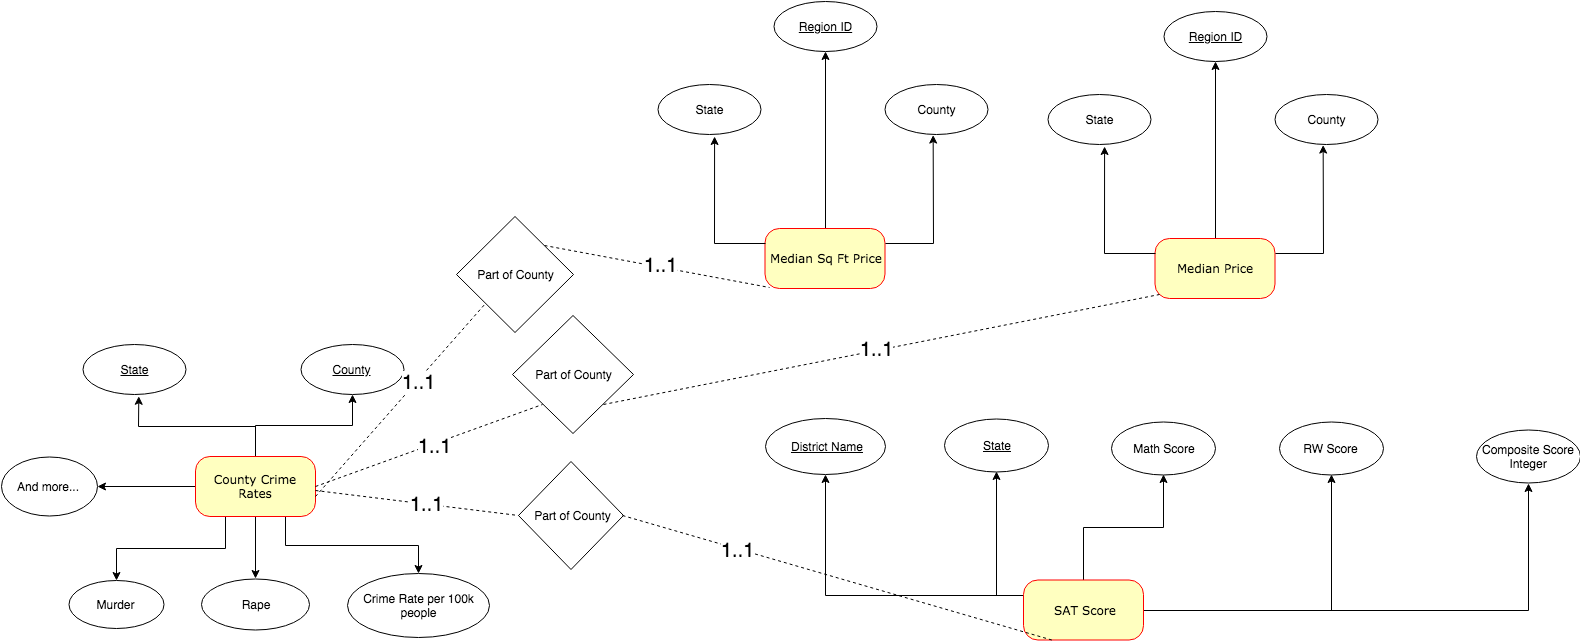
\includegraphics[width=\linewidth]{ERDiagram}
\section*{Features To Be Implemented}
\begin{itemize}
    \item Pick a state
    \item Pick a county
    \item Rank county by:
    \begin{itemize}
        \item Avg. SAT score
        \item Median home prices
        \item Median home prices per sq. ft
    \end{itemize}
    \item Query by:
    \begin{itemize}
        \item Price range
        \item High quality Schools (SAT scores)
        \item Crime rates (can also sort by type of crime)
    \end{itemize}
    \item Select county and show map of county
\end{itemize}
\section*{Possible Additional Features}
\begin{itemize}
    \item Weather data included
    \item Map
    \begin{itemize}
        \item High School pins on map
        \item Interactive Map
    \end{itemize} 
\end{itemize}
\section*{Technology and Tools}
MySQL, Node.js, Angular/React, HTML, AWS (tentative)
\section*{Member Responsibilities}
\begin{itemize}
    \item Frontend
    \begin{itemize}
        \item Andrew Si - Querying crime rates and house data
        \item Dan Truong - Querying scores and states/geographic locations data
    \end{itemize}
    \item Backend
    \begin{itemize}
        \item Harsha Uppili - will work with both zillow datasets and MA, FL, NY1, NY2, TX
        \item Jeffrey Zhou - will work with crime dataset, VA, GA, NC, IL, PA, NY    
    \end{itemize}
\end{itemize}
\end{document}
\end{document}